\documentclass{minimal}
\usepackage{tikz}

\begin{document}

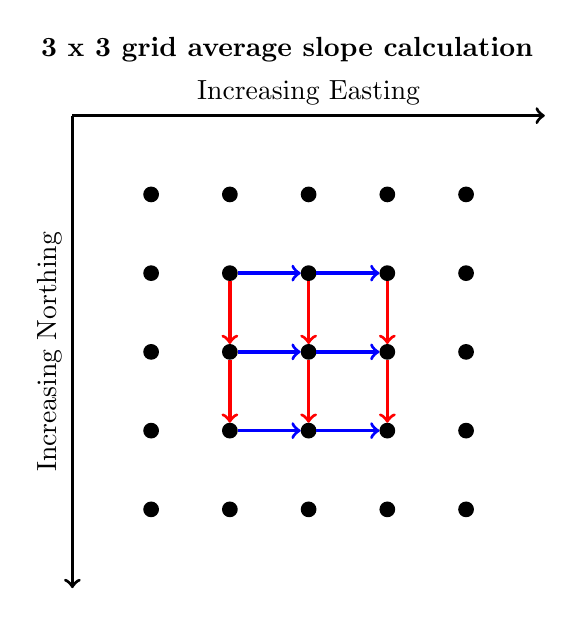
\begin{tikzpicture}

%draw external reference
\draw[<-,black,very thick] (0,0)--(0,6) node[midway,above,sloped]{Increasing Northing};
\draw[->,black,very thick] (0,6)--(6,6) node[midway,above,sloped]{Increasing Easting};

%label figure
\node[above] at (current bounding box.north) {\textbf{3 x 3 grid average slope calculation}};

%draw grid of points
\foreach \x in {1,...,5}
	\foreach \y in {1,...,5} 
       {
    	\fill (\x,\y) circle (0.1);
    	}
%draw vertical arrows    	
\foreach \x in {2,...,4}
	\foreach \y in {2,...,3} 
    	{ 
      	\draw[->,red,very thick] (\x,\y + .9)--(\x,\y + .1);
		}
%draw horizontal arrows    	
\foreach \x in {2,...,3}
	\foreach \y in {2,...,4} 
    	{ 
      	\draw[->,blue,very thick] (\x + .1,\y)--(\x + .9,\y);
		}		
		
\end{tikzpicture}

%insert space between graphics
\vspace{20mm}

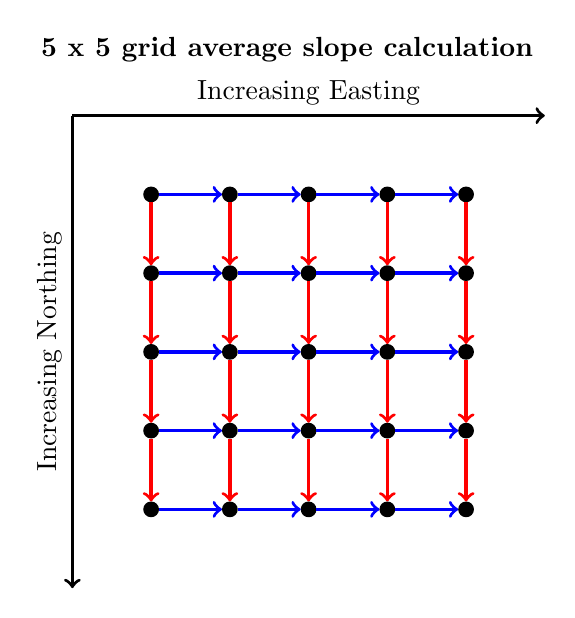
\begin{tikzpicture}

%draw external reference
\draw[<-,black,very thick] (0,0)--(0,6) node[midway,above,sloped]{Increasing Northing};
\draw[->,black,very thick] (0,6)--(6,6) node[midway,above,sloped]{Increasing Easting};

%label figure
\node[above] at (current bounding box.north) {\textbf{5 x 5 grid average slope calculation}};

%draw grid of points
\foreach \x in {1,...,5}
	\foreach \y in {1,...,5} 
       {
    	\fill (\x,\y) circle (0.1);
    	}
%draw vertical arrows    	
\foreach \x in {1,...,5}
	\foreach \y in {1,...,4} 
    	{ 
      	\draw[->,red,very thick] (\x,\y + .9)--(\x,\y + .1);
		}
%draw horizontal arrows    	
\foreach \x in {1,...,4}
	\foreach \y in {1,...,5} 
    	{ 
      	\draw[->,blue,very thick] (\x + .1,\y)--(\x + .9,\y);
		}		
		
\end{tikzpicture}


\end{document}